\newpage
\section{Question 6}
	\subsection{Inverse Kinematics}
	\subsubsection{Theoretical Method}
	In Question 3 we used forward kinematics to derive the Transformation matrix ($^{0}T_{6}$) for this robot arm with respect to our assumed "zero" coordinate system (see Figure 2).\\\newline\vspace{3mm}
	Our aim for this question is to derive the transformation matrix specific to two separate end effector points ($P_{e_{a}}$ $P_{e_{b}}$) which can be done in two ways.\\\newline\vspace{3mm}
	One method (as mentioned in Question 3) could be to apply another transformation matrix $^{w}A_{0}$ and then continue simultaneously equating.\\newline\vspace{3mm}
	
	According to our method we know that our $Z_{0}$ points are based 253 higher than the $Z_{w}$ points in space and rotated about the Z axis by $\pi/2$. We need to account for this by modifying our end effector point values from:\\newline\vspace{3mm}
	
	$P_{e_{a}} = (0, 490, 40)$\\
	$P_{e_{b}} = (0, 490, 120)$\\
	\vspace{newline}
	To:\\
	$P_{e_{a}} = (0, 490, -213)$\\
	$P_{e_{b}} = (0, 490, -133)$
	
	Since our end effector must point vertically downwards our $\sum\theta = -\pi/2$ in order to achieve this. We then simultaneously equate this with our equations for $P_{e_{x}}$ and $P_{e_{y}}$ with their equivalent values from our transformation matrix $^{0}T_{6}$. Substituting $\theta_{1} = \theta_{4} = \theta_{6} = 0$ (as we do not rotate around any axis parallel to the $Z_{0}$ axis) we can solve for $\theta_{2}, \theta_{3}, $ and $\theta_{5}$.
	
	We do this once to find all the angles for Point A and again for all the angles for point B. We can then compare these angle values with the simulator jkoint angle readings in Q6 Part B.
	
		\subsubsection{Results}
		Our Matlab output looks as follows:\\
	sa2 =
	
\hspace{20mm}	-133.57970015587177746184941710562\\
\hspace{20mm}	-56.676681927833899035216072316143\\
	
	
	sa3 =\\
	
\hspace{20mm}	166.90301822803787842663334478947\\
\hspace{20mm}	13.096981771962121573366655210527\\
	
	
	sa5 =\\
	
\hspace{20mm}	-123.32331807216610408729072583881\\
\hspace{20mm}	-46.420299844128225660657381049333\\
	
	
	sb2 =\\
	
\hspace{20mm}	-121.68117590050949105729393864272\\
\hspace{20mm}	-45.154934789134486545751233766901\\
	
	
	sb3 =\\
	
\hspace{20mm}	166.52624111137500451154270487582\\
\hspace{20mm}	13.473758888624995488457295124181\\
	
	
	sb5 =\\
	
\hspace{20mm}	-134.84506521086551657675556438805\\
\hspace{20mm}	-58.318824099490512065212859512228\\
	
	We can interpret this as Points A and B can each have two theoretical values for the angles (i.e. two possible configurations) to reach the desired end effector pose.
	
	\noindent
	\begin{table}[position = here]
		\begin{centering}
			\begin{tabular}{||c|c|c|c||}
				\hline \rule[-2ex]{0pt}{5.5ex} \color{red}\bf{Point} & \color{red}\bf{$\theta_{2}$}		&	\color{red}\bf{$\theta_{3}$}	&	\color{red}\bf{$\theta_{5}$}\\ 
				\hline \rule[-2ex]{0pt}{5.5ex} $P_{e_{a}}$ Path 1 & -56.677	&	13.096		&	-46.420\\
				\hline \rule[-2ex]{0pt}{5.5ex} $P_{e_{a}}$ Path 2 & -133.579	&	166.903	&	-123.323\\
				\hline \rule[-2ex]{0pt}{5.5ex} $P_{e_{b}}$ Path 1 & -45.155	&	13.473	&	-58.319\\
				\hline \rule[-2ex]{0pt}{5.5ex} $P_{e_{b}}$ Path 2 & -121.681	&	166.526&	-134.845\\
				\hline 
			\end{tabular}\\
		\end{centering}
		\begin{flushleft}
			\caption [Angles] {Potential Angle Values for End Effector Positions A and B}
		\end{flushleft}
	\end{table}
	\subsubsection{Code Listing}
		See Appendix A [9.5]
		
	\subsection{Simulation}

	\begin{figure}[position = here]
		\begin{centering}
			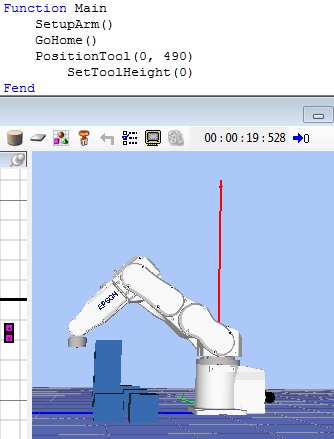
\includegraphics[scale=0.5]{Q6b_a_sim}\\
			\caption [SIMA1]{Simulator Point A}
		\end{centering}
	\end{figure}

	\begin{figure}[position = here]
		\begin{centering}
			\includegraphics[scale=0.5]{Q6b_a_Angles}\\
			\caption [SIMA1]{Simulator Point A Angles}
		\end{centering}
	\end{figure}

	\begin{figure}[position = here]
		\begin{centering}
			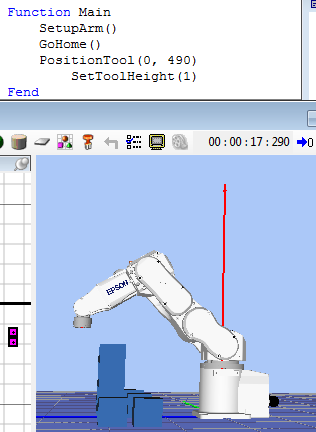
\includegraphics[scale=0.5]{Q6b_b_sim}\\
			\caption [SIMB1]{Simulator Point B}
		\end{centering}
	\end{figure}

	\begin{figure}[position = here]
		\begin{centering}
			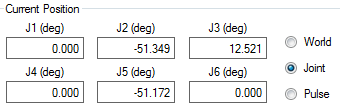
\includegraphics[scale=0.5]{Q6b_b_angles}\\
			\caption [SIMB2]{Simulator Point B Angles}
		\end{centering}
	\end{figure}
	